\chapter{Infrastructure as Code}
\label{cha:iac}
Infrastructure as Code (IaC) is a concept to automate system creation and change management with techniques from software development. Systems are defined in a Domain Specific Language (DSL), which gets interpreted by a tool, which creates an instance of the system or applies changes to it. IaC defines predefined, repeatable routines for managing systems. IaC descriptors are called templates, cookbooks, recipes, or playbooks, depending on the IaC tool. In the further course, the IaC descriptors will be called templates. The DSL allows to define resources of a system such as network, storage, and routing descriptively in a template. The DSL abstracts the developer from system specific settings and provides a way to define the system with as little configuration as possible\cite{Morris2016}. \\

The term \mentionedtext{system} is used as a general description, whereby in the context of IaC, a system can be anything, which can be described via a DSL. The term \mentionedtext{environment} is also used as a general description for a habitat for one or more systems.  

\section{The Need for Infrastructure as Code}
\label{sec:iac-need}
In the so called iron age, the IT systems were bound to the physical hardware, and the setup of such a system and its change management were a long term, complex, and error prone process. These days, we call such systems legacy systems. In the cloud age, the IT systems are decoupled from the physical hardware, and in the case of PaaS, they are even decoupled from the operating system. The IT systems are decoupled due to the fact, that cloud providers cannot allow their customer to tamper with the underlying hardware and operating system. In general, the hardware resources, provided by a cloud provider, are shared by multiple customers\cite{Morris2016}. \\

With IaC it is possible to work with so called Dynamic Infrastructure Platforms (DIPs), which provide computing resources for a system, whereby the developers are completely abstracted from the underlying infrastructure. DIPs have the characteristic to be programmable, are available on demand, and provide self service mechanisms, therefore, we need IaC to work with such infrastructures. Systems deployed on DIPs are flexible, consistent, automated, and reproducible\cite{Morris2016}. \\

The term \mentionedtext{infrastructure} is used as a general description for the foundation of systems, which provides any kind of resources the systems can consume. \\

Enterprises, which stuck to legacy systems, face the problem that technology nimble competitors can work with their infrastructures more efficiently, and therefore can demand lower prices from their customers. This is due to the IaC principles, which are discussed in Section \vref{sec:iac-principles}. Over a short period of time, enterprises will have to move to IaC and away from their legacy systems to stay competitive. The transition process could be challenging for an enterprise, because they lose control over the physical hardware, and maybe also over the operating system. Maintaining legacy systems has the effect, that someone is close to the system, and almost everything is done manually. IaC has the goal to automate almost everything, which requires trust for the cloud providers, which provide the infrastructure and the tooling. A well known problem, which enterprises will face, is the so called Automation Fear-Spiral, which is shown in Figure \vref{fig:automation-fear-spiral}.

\begin{figure}[htbp]
	\centering
	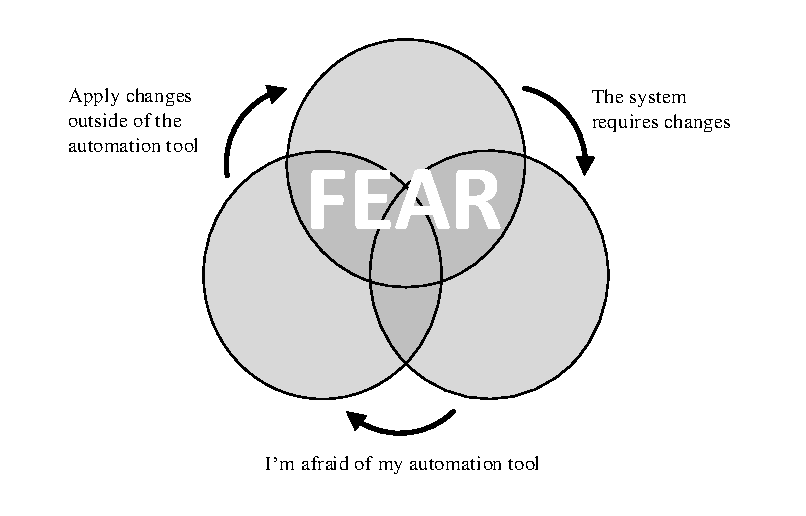
\includegraphics[scale=1]{images/automation-fear-spiral.pdf}
	\caption{Automation Fear-Spiral}
	\label{fig:automation-fear-spiral}
\end{figure} 

Because of no trust for the automation, changes are applied manually to the systems, and outside the defined automation process. If the system is reproduced, definitions maybe missing in the templates, which leads to an inconsistent system. Therefore, enterprises have to break this spiral to fully profit from IaC \cite{Morris2016}. \\

When enterprises have moved their legacy systems to IaC, they can not only manage their systems faster, they also can profit from the principles of IaC as discussed in Section \vref{sec:iac-principles}. With IaC, systems are less complicated to manage, changes can be applied without fear, and the systems can easily be moved between environments. This provides the enterprises with more space to maneuver, whereby the systems can become more complex, but still easy to manage, and the systems can be defined and created faster, which could lower costs.    

\section{Principles of Infrastructure as Code}
\label{sec:iac-principles}
The principles of IaC solve the problems of systems of the iron age. In the iron age the creation and maintenance of systems were a long term, complicated, and error prone process, which consumed a lot of resources and time. With the decoupling of the physical hardware from the systems, the creation and maintenance of systems has become simple, due to the abstraction layer provided by the IaC DSL and tooling. 

\subsection{Systems are Reproducible}
\label{sec:iac-principles-reproducibility}
With IaC, systems are reproducible. It is possible to reproduce a whole system or parts of it effortlessly. Effortless means, that no tweaks have to be made to the templates or during the reproduction process, and there is no need for a long term decision process about what has to be reproduced and how to reproduce it. To be able to reproduce systems effortlessly is a powerful capability, because it can be done automatically, consistently and with less risk of failures. The reproducibility of a system is based on reusable templates, which expose parameters, whereby the parameter values are defined for a specific environment. Figure \ref{fig:reproduce-infrastructure} illustrates the reproduction of a system into two different environments, whereby the IaC tooling reads the templates and sets the defined parameters with the environment specific values\cite{Morris2016}.

\begin{figure}[htbp]
	\centering
	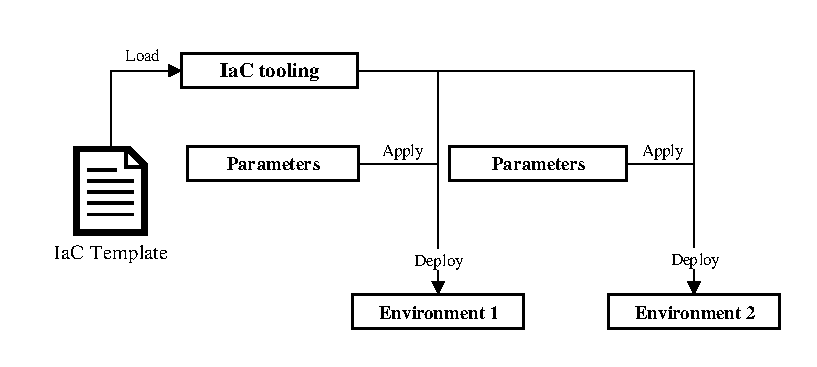
\includegraphics[scale=1]{images/reproduce-infrastructure.pdf}
	\caption{Schema of a parametrized system reproduction}
	\label{fig:reproduce-infrastructure}
\end{figure} 

\subsection{Systems are Disposable}
\label{sec:iac-principles-disposable}
Another benefit of IaC is, that systems are disposable. Disposable means, that systems can be easily destroyed and recreated. Changes made to the templates, describing a system, don't have to be applied on an existing system, but can be applied by destroying and recreating the system. A requirement for a disposable system is, that it is understood, that systems will always change. Other systems, relying on a disposable system, need to address the fact, that the system could change at any time. Systems must not fail, because a disposable system disappears and reappears again because of a redeployment \cite{Morris2016}.

\subsection{Systems are Consistent}
\label{sec:iac-principles-consistency}
Systems managed with IaC are consistent, because they are defined via parametrized templates, and are created by a predefined workflow. All system instances are an instance of the system templates, with the little configuration differences defined by parameters. As long as changes of a system are managed by IaC, the system will stay consistent, and the automation process can be trusted. \\

Listing \vref{src:iac-template-docker-compose} shows an example for an IaC template, which defines a Docker Compose system for hosting a Wildfly server instance. This system can consistently be reproduced on any environment supporting Docker, Docker Compose, and providing values for the defined parameters\cite{Wildfly2017, DockerCompose2018}. \\

\begin{code}
	\yamlFile{\sourceDir/iac-docker-compose.yml}
	\caption{Example for an IaC template of Docker Compose}
	\label{src:iac-template-docker-compose}
\end{code}

\subsection{Actions are Repeatable}
\label{sec:iac-principles-repeatability}
Building reproducible systems means, that any action applied to the system has to be be repeatable. Without repeatability, the automation cannot be trusted and systems wouldn't be reproducible. An instance of a system in one environment has to be equal to any other system instance in any other  environment, except for the configurations defined by parameters. If this is not the case, then a system is not reproducible, because it will have become inconsistent \cite{Morris2016}. \\

IaC is a concept which makes it easy to manage systems in the cloud age. Enterprises can make use of IaC to make their existing systems more reliable, consistent and easier to manage. Nevertheless, before an enterprise can profit from IaC, it has to apply clear structures to their development process, as well as sticking to the automation process provided by the IaC tooling. For experienced administrators, who are used to maintain systems manually, it could be sometimes hard to understand why they are not supposed to perform any actions on the system manually anymore. Being capable to reproduce a system at any time in any environment effortlessly, or applying changes on an existing system in a predefined and consistent manner, makes enterprises very flexible and fast. Enterprises will not have to fear future changes in requirements and technologies of their systems anymore, because they are abstracted from the technologies by the DSL and IaC tool. \\

The following chapter will discuss containerization with Docker, which is very popular tooling for isolating processes on a Linux host. Docker strongly relies on the principle of IaC, and therefore can be seen as a IaC tool for managing isolated processes.    



